% !TeX root = ../libro.tex
% !TeX encoding = utf8

\chapter{Conceptos básicos}

Este capítulo tiene el objetivo de introduccir los conceptos básicos sobre Informática Gráfica y OpenGL, tales como aquellos relacionados con la representación computacional de objetos ``3D'' y algunos resultados matemáticos usados, del campo de la topología diferencial. Dichos conceptos se han obtenido de las referencias \cite{KhronosWiki} y \cite{LearnOGL}, junto con el conocimiento adquirido de la asignatura Informática Gráfica y las del departamento de Geometría y Topología.\\
\\Se sugiere la lectura de las definiciones de ``sistema coordenado'' (o carta), ``variedad topológica'', ``variedad diferenciable'' y ``función de Morse'' del apartado de \textbf{Conceptos Previos} de la parte I, con el objetivo de orientar al lector en el sentido matemático que subyace en esta parte informática (aunque no es necesario si ya se tiene una ligera idea).\\

\begin{definicion} Una \textbf{GPU} es una unidad de procesamiento gráfico, especialmente diseñada para la visualización de elementos gráficos (ya sean $2$D o $3$D mediante una proyección), en particular para el cálculo vectorial. Realizar este tipo de cálculos en esta unidad reducirá el uso de CPU, se completarán en menor tiempo e incluso con mayora paralelismo (contiene una gran cantidad de unidades de cálculo en coma flotante).\\
\\Además, normalmente suele albergar una unidad de almacenamiento temporal (VRAM), para reducir el nº de comunicaciones a través del bus de datos (extremadamente lento).
\end{definicion}

\begin{definicion} Una \textbf{primitiva} es el objeto básico de visualización. Pueden ser puntos, segmentos, patrones de segmentos, polígonos y patrones de polígonos. En nuestro caso las primitivas a usar serán triángulos.
\end{definicion}

\begin{definicion} Entenderemos por \textbf{malla} una malla de triángulos, que es un conjunto de triángulos que aproximan a una cierta superficie. Cuando nos referimos a la \textbf{malla inicial}, hablamos de la aproximación del cuadrado $[0,1]\times[0,1]\subset \R^2$ para un cierto número de triángulos (se calcula una cuadrícula y se dividen por las diagonales para obtener los triángulos).\\
\\Una malla se dirá que está \textbf{indexada} si para definir los triángulos se proporcionan primero los vértices sin repetirlos, y después se definen los triángulos en base a los índices de los vértices. Por ejemplo, para un cuadrado tendríamos los vértices $(0,0)$ $(1,0)$ $(1,1)$ $(0,1)$, pues si los numeramos del $0$ al $3$, el triángulo de la diagonal inferior se definiría como $(0,1,3)$, y el superior $(1,2,3)$. Esta técnica reduce el número de vértices a almacenar y procesar, ya que para el caso normal se deberían definir los vértices para cada triángulo a dibujar.
\end{definicion}

\begin{definicion} La \textbf{representación de fronteras} (boundary representation o B-rep) consiste en la aproximación de un cuerpo topológico o geométrico mediante una malla. De esta manera se aproximan las posibles caras del objeto, pero para ello hay que tener en cuenta la posibilidad de definir una orientación, necesaria para definir cual es la parte interior/exterior de la cara. Aquellos objetos que no sean orientables no podrán visualizarse correctamente, en cuanto a iluminación, ya que sus caras interior y exterior coinciden (deberán aproximarse con más de una representación).
\end{definicion}

\begin{definicion} La acción \textbf{teselar} consiste en subdividir una primitiva en primitivas más pequeñas, para así poder aproximar mejor la superficie que se quiere representar. En el caso de OpenGL, para realizar la teselación es necesario especificar los respectivos niveles de teselado.
\end{definicion}

\begin{definicion} El \textbf{nivel de teselado en un lado} (outer) es el número de partes en el que se dividirá el lado para el teselado de la primitiva. Por ejemplo, si el nivel es $3$ para un cierto lado, dicho lado se dividirá en $3$ partes iguales, que serán los lados de los nuevos triángulos.
\end{definicion}

\begin{definicion} El \textbf{nivel de teselado en el interior} (inner) es el número de partes en el que se dividirá la primitiva hacia el interior. Por ejemplo, si el nivel es $3$ para una cierta primitiva, dicha primitiva se dividirá en $3$ niveles hacia el baricentro.
\end{definicion}

\begin{figure}[h]
  	\centering
  	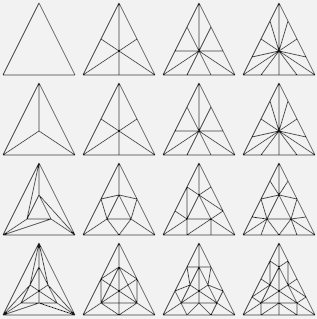
\includegraphics[width=0.4\textwidth]{nivel_tess}
	\caption{Niveles de teselado del $1$ al $4$: outer en horizontal (todos los lados por igual) e inner en vertical.}
  	\label{fig:nivel_tess}
\end{figure}

\begin{definicion} Un \textbf{shader} es un tipo específico de programa informático que se ejecuta en la GPU. Su uso principal es el cálculo de gráficos. En OpenGL existen los siguientes tipos de shaders:
	\begin{itemize}
		\item Vertex shader: se ejecuta para cada vértice de entrada. Se utiliza para podificar cada vértice.
		\item Tessellation control shader: tiene de entrada una primitiva y devuelve un patch (conjunto de primitivas), según los niveles de teselado.
		\item Tessellation evaluation shader: similar al vertex shader pero diseñado para la salida del tessellation control shader.
		\item Geometry shader: tiene de entrada una primitiva y devuelve varias primitivas.
		\item Fragment shader: después del rasterizado (pasar de gráfico vectorial a píxels), se ejecuta para calcular el color de cada fragmento de triángulo.
		\item Compute shader: etapa utilizada para realizar cáculos en general. No suele usarse para el renderizado en sí (no se ha utilizado en el proyecto).
	\end{itemize}
\end{definicion}

\begin{definicion} La \textbf{curvatura de Gauss} (K) es una función que a cada punto de una superficie $S$ le asigna un valor de $\R$. Indica el tipo de geometría entorno al punto:
	\begin{itemize}
		\item $K_p = 0$, euclídea, localmente es $\R^2$.
		\item $K_p > 0$, esférica, localmente es una esfera de radio $R = \frac{1}{\sqrt{K_p}}$.
		\item $K_p < 0$, hiperbólica, localmente es un espacio hiperbólico de cruvatura $K_p$.
	\end{itemize}
La curvatura de Gauss se ha calculado de la siguiente forma \cite{Wolfram}:
		$$K_{x(u,v)} = \frac{det(x_{uu}, x_u, x_v) det(x_{vv}, x_u, x_v) - [det(x_{uv}, x_u, x_v)]^2} {[|x_u|^2|x_v|^2 - <x_u, x_v>^2]^2} (u, v)$$
	que es la curvatura de Gauss en el punto $x(u, v)$, con $x$ carta de la superficie $S$. Existen muchas maneras distintas de calcularla, pero esta es la que nos favorecerá para su correcta obtención mediante los árboles de expresión.
\end{definicion}

\endinput
%------------------------------------------------------------------------------------
% FIN DEL CAPÍTULO. 
%------------------------------------------------------------------------------------
